\RequirePackage{ifluatex, ifxetex} % these are for the portability of this example - can be omitted in any actual document made for a certain engine

\ifnum 0\ifxetex 1\fi\ifluatex 1\fi>0
\else
  % only needed for using Greek letters outside math when running PDFLaTeX - leave out otherwise
  %\PassOptionsToPackage{LGR}{fontenc}
  %\RequirePackage{textgreek}
\fi


\documentclass[twoside,draftfooter]{tutthesis} % see appendix for list of options

\pagestyle{headings} % Adds titles to the header


% ifnameyear is defined to demonstrate both versions in a single file. You may leave it out and simply use one version throughout your file.
\newif\ifnameyear
\nameyearfalse



% ==============
% Basic packages
% ==============
% You should use these unless you really know what you're doing

\ifnum 0\ifxetex 1\fi\ifluatex 1\fi>0
\else\usepackage[utf8]{inputenc}
\fi

\usepackage[finnish,english]{babel} % The language of the thesis last

% If you are working with a minimal LateX distribution, you may have to install some extra packages. Make sure that at least babel-finnish (available in e.g. texlive-lang-european) and the basic fonts (e.g. texlive-fonts-recommended) are installed.

\usepackage[fixlanguage]{babelbib} % You should use this unless you are using biblatex. Add option fixlanguage if you're writing in English (the thesis writing guide is asymmetric, requiring Finnish theses to have e.g. 'eds.' for sources in English, while requiring English theses to have all such parts in English)

\ifnameyear\usepackage{natbib} % add option longnamesfirst if you want to have full author list with first citation
\else\providecommand{\citep}{\cite} % This template is written using \citep to get name-year citations right, and in numerical mode the command is here aliased to the standard \cite. If you use numbered citations, leave this out and use \cite
\fi


% ===============
% Useful packages
% ===============
% Packages which are not required for a thesis that follows guidelines, but may be convenient or necessary in common cases

\usepackage{microtype} % subtle but nice improvements to how text is printed

\usepackage{textcase} % may be used to keep parts of title lowercase

\usepackage{array}
\usepackage{tabularx} % e.g. multiline cells
%\usepackage{calc} %for performing length arithmetic such as column width = text width minus some other width
%\usepackage{longtable} % for tables spanning multiple pages

%\usepackage{psfrag} % editing ps files
%\usepackage{subfig} % parallel small figures a,b,c,...
%\usepackage{rotating} % for rotating e.g. full-page figures

%\usepackage{siunitx} % nice formatting for combinations of number and unit
\usepackage{amsopn} % For operator names; not necessary if amsmath is used
%\usepackage[fleqn]{amsmath} %Extensions to math handling; if you use this, you should use e.g. gather instead of equation due to a hyperref bug

\usepackage{listings} %Typesetting code
\lstset{basicstyle=\footnotesize\ttfamily, numbers=left}
\renewcommand{\lstlistingname}{Program} % Program if you're writing in English
% If you want non-ASCII characters (e.g. in comments), check out the listingsutf8 package

\ifnum 0\ifxetex 1\fi\ifluatex 1\fi>0
  \usepackage[math-style=ISO]{unicode-math} % must not precede amsmath and most other math and font related packages
\else
  %\usepackage{bm} % The \bm command is used for bold italic variables used in some fields not to be used with unicode-math
  %\usepackage[helvratio=1]{newtxtext} \usepackage{newtxmath}% some recommend the newtx fonts
  \usepackage{textcomp} % symbols like \textdegree
\fi


% ===========================
% Bibliographic information
% ===========================
% These must be set before loading pdfx or beginning document
\author{Luong Dang Hai}
\title{The Ethereum blockchain: Use cases for social finance applications}
\datethesisapproved{2018}{10}{30} % year, month, day; no leading zeroes; submitted for bachelor's theses and thesisapproved for master’s
\thesistype{Bachelor’s thesis} % Do not use ASCII apostrophe ' as it will not be substituted with the correct one (’) in the PDF metadata. Note that there are both short version (this) and a long one - "Master’s" vs. "Master of Science"
\major{Information and Communication Technology}
\programme{Bachelor’s Degree Programme in Science and Engineering} % Note apostrophes on all fields for PDF metadata
\keywords{blockchain, smart contract, solidity, ethereum, finance}

\examiner{Professor Marko Helenius} %\and for plural
\datetopicapproved{2018}{9}{11}% only for master’s theses


% Packages that need to be loaded late
% ----------------------------------------------
\usepackage[a-2u]{pdfx} % If you're using PDFLatex and your version of pdfx is not recent enough, you may run into the inputencoding bug. In that case, load inputenc after pdfx (and replace any non-ASCII characters in the metadata with e.g. \"{a})

%\usepackage{hyperref} % This must (usually) be the last package you load - load this OR pdfx (which also loads hyperref). Usage of pdfx would be nice, but if you have issues with that you may fall back to just hyperref



\begin{document}

\maketitle


%First, the abstract in the language of the thesis (no language selection). Note that most fields are already defined

\thesisdescription{Bachelor of Science and Engineering Thesis}
\begin{abstract}
Transaction-based activities existed since humanity was known, which can range from trading goods to information. Together with the flow of time, the requirements and complexity of transactions demand a role called middleman, acting as an escrow to ensure the transaction was made according to all parties' wish, which means trust becomes an important part of all transactions. However, the reliance of trust in this modern technological age has shown signs of limitations and mistrust was found in history, since the middleman cannot always be fully trusted. Hence, a new model of transaction needs to be invented to eliminate the need of middleman and trust in order to provide more robust transactions which lead to better efficiency in business and relationship.

Cryptography was one of computer science's field which studies the process of making sure the information is secure, unaltered and non-reputable until it reaches the receiver. This technology has shown its usefulness and importance throughout history, which makes cryptography to be a viable solution for creating a new model of transaction, of which is called "Blockchain" nowadays.

This bachelor's thesis studies the Ethereum blockchain, which is one of the most developed and widely-accepted blockchain implementation, to find its benefits in social financial applications, specifically providing transparency and availability of data to all parties. The research is done by implementing a smart contract on the Ethereum blockchain which will allow reading and writing data to Ethereum blockchain. With this smart contract, transactional data will be transparent, unalterable and guaranteed available for everyone. 
\end{abstract}


\chapter*{Preface}

I would like to thank my employer Bankify Oy for suggesting this bachelor thesis and making this thesis possible. I want to also thank to my supervisor, Marko Helenius, for the aid I was given to improve this thesis.

\vspace{2\baselineskip}

In Tampere, Finland, on 15 Sep 2018

\vspace{2\baselineskip}

Luong Dang Hai



\tableofcontents

\listoffigures
%\listoftables



\chapter*{List of Symbols and Abbreviations}

% This is not a "proper" table, so no table environment

% Suppressed left colsep; 20% - 1 x colsep; right colpsep; left colpadding; 80% - 1 x colpadding; suppressed right colpadding
\begin{tabular}[h]{@{} p{0.2\textwidth-\tabcolsep} p{0.8\textwidth-\tabcolsep} @{}}
TX & Transaction \\
ETH & Ether, the currency of the Etherum blockchain \\
TUT & Tampere University of Technology \\
URL & Uniform Resource Locator 
\end{tabular}

\begin{tabular}[h]{@{} p{0.15\textwidth-\tabcolsep} p{0.85\textwidth-\tabcolsep} @{}}
$a$ & acceleration \\
$\mathbf{F}$ & force \\
$m$ & mass
\end{tabular}

The abbreviations and notations used in your thesis are defined collectively at the start of the thesis, and when they appear in the body for the first time.
Parentheses are used with abbreviations then.


% It may be useful to break the chapters into their own files and then do eg. \include{01-introduction} or \include{C-resultsdiscussion}

\chapter{Introduction (Work in Progress)}
\label{ch:Introduction}

Making transactions cannot be avoided in the technology and internet-based era. Internet users need to get the necessary work information, check bank account balances, purchasing items online, participate on voting, signing electrical contracts or papers,... All of the mentioned activities require a middleman individual or organization to help facilitating, validating and confirming. This current model of relying on the trust with middleman causes difficult issues (TO DO: add some facts about scams, unavailability of the current middle man bases transaction). Thus, a non-escrow transaction model needs to be derived to solve this issue. Nick Szabo proposed "smart contract" as an improved solution to eliminate the use of middleman (TO DO: insert reference to Nick Szabo's paper: \href{http://www.alamut.com/subj/economics/nick_szabo/smartContracts.html}{Smart Contracts: Building Blocks for Digital Markets}) (TO DO: read the above paper and then create a link to Bitcoin's blockchain invention by Satoshi Nakamoto)

Then tell a story an transition from Bitcoin to Ethereum and then link Ethereum's white paper here. Then tell the smart contract concept in Ethereum

\chapter{Background}
\label{ch:background}

This chapter explains the key concepts of a blockchain, a new blockchain feature called smart contract and introduces a platform that provide the capability to develop one which is the Ethereum blockchain. Understanding the key ideas is the prerequisite to understand: i) the revolutional idea of blockchain; ii) the solutions proposed in later chapters.

\section{Blockchain Definitions}

A blockchain is a structure to store data in a continuously growing list of records, which are also referred to as "blocks" \citep{RefWorks:doc:WhatIsBlockChain}. These "blocks" are linked and secured by cryptography.

A blockchain can be compared to a book which can add pages to itself infinitely. Each block is similar to a page, which contains a page number to identify itself. All pages are linked to each other by the book spine, and each page number implies that the next page is certainly the current page number plus one. With this setup, the reader can easily jump to the page as needed, and navigate between pages. A blockchain is constructed in a similar way as that book while the page numbers are replaced by unique identifiers such as a hash value, the book spine is removed and instead each page contains the identifier for the previous page \citep{RefWorks:doc:BlockchainBasicsBook}.

\subsection{Content creation on the blockchain}
\label{contentCreationOnBlockchain}

Content addition to the blockchain is similar to new content addition to a book. For example, anyone can get a digital version of a thesis, write edit and annotate. There has to be a solution to validate which printed out versions of that thesis is the original one. One such solution is comparing all copies of the same book. If the same page is showing different content between versions, the majority which hold the same content will be correct. To the blockchain context, everyone will have the same copy of data and have the right to add new content to it. Each time content is added there will be a broadcast event to everyone, each of whom can verify the data and the majority will decide the next set of data will be added to a new block \citep{RefWorks:doc:BitcoinWhitepaper}.

Blockchains improve the content creation by allowing more complex "content" which can be added into itself. These "contents" can be transactions data, messages, texts, conditions and even computer programs, or scripts which run when the conditions are met.

\subsection{Blockchain's capabilities}
\label{blockchainCapabilities}

From the definition and the mechanism of content creation mentioned above, it is derived that a blockchain is able to:

\begin{itemize}
    \item Transfer values, such as electronic cash \citep{RefWorks:doc:BitcoinWhitepaper}.
    \item Exchange message to each others as a form of signed message (to which the receiver is able to verify the sender) \citep{RefWorks:doc:EthereumWhitepaper}
    \item Store records of data such as company shares, bonds, ... \citep{RefWorks:doc:SecuritiesOnBlockchain}
    \item Run optional scripts each time a condition is met \citep[s.~20]{RefWorks:doc:MasteringBlockchain}
\end{itemize}

For the purpose of this thesis, finding use cases for a social finance application, only the data storing and script executing will be discussed. This is due to the nature of a computer application: i) Running business logic, and ii) Storing users' data.

\subsection{Transparency and democracy}

These capabilities mentioned in section \ref{blockchainCapabilities} can be found in current systems. For example, the records of company shares are saved in that company, legal authority. Those middlemans make sure that all shareholders's stake are recorded correctly. Each time one needs to transfer the shares, all those middlemans need to be notified and then they will then verify and execute the transfer. Those outlined steps might be broken if a chain is corrupted or a human error occured.

A blockchain prevents these issues with the reliability of data existence, automatic agreement bindings and no authority in control. All participants in a blockchain will keep a record of that company's shares and share transfer will be handled by a smart contract automatically \citep{RefWorks:doc:BlockchainProtocolInClinicalTrials}. Anyone in the entire world can safely make an agreement to each other without actually meet or know before hand, since the rules and execution of a smart contract are automated.  Each time new data is requested to record, the whole network will verify it with cryptography. Later, the data will be immutable, extremely hard to temper with \citep{RefWorks:doc:BitcoinWhitepaper}\citep{RefWorks:doc:EthereumWhitepaper}. Furthermore, no one owns the system. Instead, it is maintained, verified and controlled by everyone who joins the network.

\section{Smart contracts}

Smart contracts are new feature of a blockchain \citep{RefWorks:doc:BlockchainInSustainableEnergySystem}, is a "computerized transaction protocol that executes the terms of a
contract" \citep{SmartContracts}. As mentioned in section \ref{contentCreationOnBlockchain}, any request to run the smart contract codes will be sent with a set of conditions. When the predefined conditions are met, the codes from the smart contract will be executed \citep{RefWorks:doc:MasteringBlockchain}.

In a traditional contract, each party will hold a copy. The judges and the legal system will enforce and make sure that the contract terms will be respected and followed. The judges and legal system, in contrast, does not exist in smart contracts. Since they are computer programs, all the rules execution are automated and enforced by computer logic.

\subsection{Smart contract innovation}

Since smart contracts are essentially computer programs \citep{Ethdocorg:EVM}, a whole new possibility has been able to be realized since more complex rules and logic can be applied thanks to smart contracts. Running smart contracts on blockchain can also be understood as running computer programs in a "world computer", since the contract will be executed anywhere in the world, which ensures the availability of the contract (zero downtime). Furthermore, since the contract execution will be made by every node joining the network, "an extreme level of fault tolerant" can be achieved \citep{Ethdocorg:EVM}.

With a smart contract, two random people on the planet, for example Anna and Bob can agree to certain terms and conditions without actually meet and know each other before hand. They do not need to spend time and money from different third party entities to formalize and legalize the contract. Instead, what is required from them is only running the smart contract, and all the rules will be automated without anyone's worry.

\subsection{Supported Platform and Availability}

Smart contract is a new an attractive feature that many modern blockchain has implemented this. Here are some popular example according to the current time of writing this thesis:

\begin{itemize}
    \item Ethereum \citep{Ethereum}
    \item Eos.io \citep{EOS}
    \item NEO Project \citep{NEO}
\end{itemize}

Each of the above mentioned platforms have its own strengths and weaknesses. However, in this thesis, a smart contract will be developed on the Ethereum blockchain due to its popularity and huge base of community and developer support.

\section{The Ethereum blockchain}

After the successful release of the first blockchain platform called \textit{bitcoin}, the whole world has been introduced and gradually accept the advantages of blockchain technology. However, the problem that \textit{bitcoin} solved was only sending electronic money between peers, and the community demands a next generation of blockchain that can achieve more, for example, running computer programs with consensus-backed security. That was the reason for the born of Ethereum blockchain to become a "programmable blockchain" in the year 2014 \citep{Ethdocorg:WhatIsEthereum}. Ethereum took a different approach to blockchain by allowing everyone to add their own operations and complexity rather than just a money transaction \citep{RefWorks:doc:MasteringBlockchain}. Therefore, Ethereum is suitable to realizing complex business logic \citep{RefWorks:doc:EthereumStateOfKnowledge}.

The design of Etherum is similar to a state machine \citep{RefWorks:doc:EthereumStateOfKnowledge}\citep{RefWorks:doc:MasteringBlockchain}\citep{RefWorks:doc:EthereumASecureDecentralizedTransaction}. Every time one wants to change the data on Ethereum, a transaction is created. The transactions will be collected and processed incrementally, each of which will describe how the data will transform from the current state to the next one, as in Figure \ref{fig:ethereum_transaction}

\begin{figure}
    \centering
    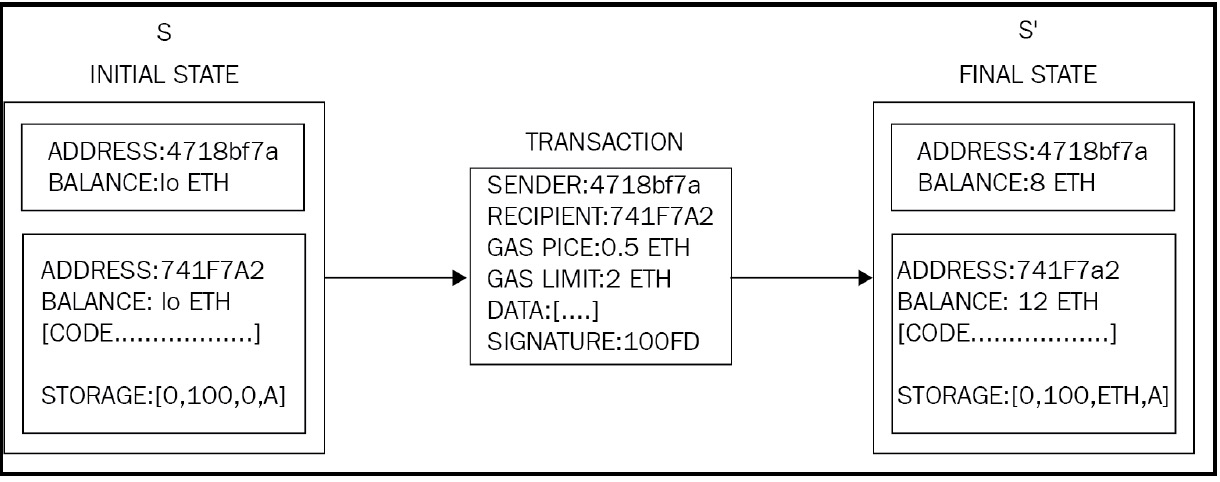
\includegraphics[width=\linewidth]{ethereum_transaction.jpg}
    \caption{Ethereum Transaction \citep{RefWorks:doc:MasteringBlockchain}}
    \label{fig:ethereum_transaction}
\end{figure}

There are currently two Ethereum network running: Ethereum Classic (ETC) \citep{EthereumClassic} and Ethereum (ETH) \citep{Ethereum}. In this thesis, the Ethereum ETH will be used to discuss and implement the smart contract due to the speculation that the later Ethereum is more popular, advanced and actively maintained. The currency from Ethereum will be refered as "Ether" after this.

\subsection{Smart contract execution on Ethereum}

In Ethereum, each smart contract has its own address after being released to the network. To run one, an user with another Ethereum address will need to initiate a transaction to the contract, which optionally contains the amount of Ether to transfer, the message to invoke some function on the smart contract, and amount of fee (GAS) to paid for the miners. The transaction will be verified by the network which consumes GAS gradually and if the transaction is invalid, the remaining fee will be refunded to the sender. Otherwise, the amount of Ether specified will be transfer and the code invocation will be activated on the transaction, which will run a specified function on the smart contract.

\chapter{Smart contract development}
\label{ch:smartcontractdev}

Smart contracts are simply programs which run on top of a blockchain network. Hence, they can be developed similarly as normal computer programs, by using programming languages to compile the logic of the software, which then after that being compiled to machine instruction in order to execute. In the Ethereum blockchain, Solidity is introduced to be one of the programming languages which have the support to compile smart contract code \citep{SolidityDocumentation}. 

Solidity is a modern language inspired by many predecessors such as C++, Python and JavaScript \citep{SolidityDocumentation}. It is built with the support for Ethereum Virtual Machine (EVM), which is the platform to execute smart contracts, hence becomes a contract-oriented programming language \citep{SolidityDocumentation}. Together with any other modern counterparts, Solidity features inheritance, statically typed and libraries to ease the development process. To understand later code examples shown in later chapters, the language's features which are contracts, function modifiers, addresses will be described in details

\section{Contracts}

Contracts can be known as the soul of Solidity, and are similar to classes in other object-oriented programming languages, with the appearance of state variables equivalent to class properties, functions to class methods. For example, Program \ref{lst:simpleContract} shows a basic contract.

\begin{lstlisting}[float,caption={A simple contract in Solidity.},label={lst:simpleContract},language=Solidity]
pragma solidity ^0.4.0;

contract SimpleStorage {
    uint storedData; // State variable
    
    function getData() public returns uint {
        return storedData;
    }
    
    function setData(uint newData) public {
        storedData = new Data
    }
}
\end{lstlisting}
\label{lst:simpleContract}

Program \ref{lst:simpleContract} shows a contract \texttt{SimpleStorage} which contains a state variable of type \texttt{uint}. This contract also provides two functions, first of which is \texttt{getData()} which returns the value of the state variable \texttt{storedData}, and the second is \texttt{setData(uint newData)} which receives a parameter of type \texttt{uint} and will set that parameter's value into the state variable

\section{Addresses}

Address is a value type in the Solidity language to denote the Ethereum address, each of which contains a 20-byte value equalling to the size of an Ethereum address \citep{SolidityDocumentation}. The address can be from a real person holding an Ethereum wallet, or another contract, since contracts also own an Ethereum address. This type \texttt{address} includes some members, which is identical to methods and property of an object in other object-oriented programming languages, such as \texttt{balance} and \texttt{transfer}. By having this special value type, it is possible to programmatically send and receive money inside an Ethereum smart contract.

\section{Function modifiers}
\label{section:functionModifiers}

Functions in Solidity contracts can have modifier to change the behavior of its own \citep{SolidityDocumentation}. With function modifiers, methods can be protected by checking a precondition before executing. Program \ref{lst:simpleFunctionModifier} shows a contract which includes a simple function modifier.

\begin{lstlisting}[float,caption={Simple function modifier in a contract \citep{SolidityDocumentation}.},label={lst:simpleFunctionModifier},language=Solidity]
pragma solidity ^0.4.0;

contract owned {
    function owned() public { owner = msg.sender; }
    address owner;

    // This contract only defines a modifier but does not use
    // it: it will be used in derived contracts.
    // The function body is inserted where the special symbol
    // `_;` in the definition of a modifier appears.
    // This means that if the owner calls this function, the
    // function is executed and otherwise, an exception is
    // thrown.
    modifier onlyOwner {
        require(
            msg.sender == owner,
            "Only owner can call this function."
        );
        _;
    }
    
    // Calls to `close` only have an effect if
    // they are made by the stored owner.
    function close() public onlyOwner {
        selfdestruct(owner);
    }
}
\end{lstlisting}

In Program \ref{lst:simpleFunctionModifier}, the contract \texttt{owned} is assigned an Ethereum address coming from the caller of the constructor function, which is included in \texttt{msg} variable, as the owner when being created. During the lifetime of the contract, the function \texttt{close()} can only be effectively executed if the caller's address is equal to the owner's address.

\section{Events}

In order to get the best out of smart contracts, there has to be a method to communicate with them from the applications, website, ... Thus, events are designed as a contract feature in Solidity. Each event contains the data denoted from the time which its contract is created. When being called, the transaction's logs will store the event. Program \ref{lst:contractEvent} and \ref{lst:eventListener} demonstrates a simple interaction from a web application with a smart contract.

\begin{lstlisting}[float,caption={Contract with Event \citep{SolidityDocumentation}.},label={lst:contractEvent},language=Solidity]
pragma solidity ^0.4.0;

contract ClientReceipt {
    event Deposit(
        address indexed _from,
        bytes32 indexed _id,
        uint _value
    );

    function deposit(bytes32 _id) public payable {
        // Events are emitted using `emit`, followed by
        // the name of the event and the arguments
        // (if any) in parentheses. Any such invocation
        // (even deeply nested) can be detected from
        // the JavaScript API by filtering for `Deposit`.
        emit Deposit(msg.sender, _id, msg.value);
    }
}
\end{lstlisting}

\begin{lstlisting}[float,caption={Listening to Event from web applications \citep{SolidityDocumentation}.},label={lst:eventListener},language=JavaScript]
var abi = /* abi as generated by the compiler */;
var ClientReceipt = web3.eth.contract(abi);
var clientReceipt = ClientReceipt.at("0x1234...ab67" /* address */);

// Pass a callback to start watching immediately
var event = clientReceipt.Deposit(function(error, result) {
    if (!error)
        console.log(result);
});
\end{lstlisting}

In Program \ref{lst:contractEvent}, contract \texttt{ClientDeposit} contains a function \texttt{deposit} which emit event \texttt{Deposit} when successfully executed. The event contains the Ethereum address of the sender, the identifier \texttt{\_id} and the amount of deposit \texttt{value}. After being compiled and deployed to the Ethereum network, an identifier called as \texttt{abi} is generated, which can be used from outside of the Ethereum network to specify the contract. In a webpage which embed the JavaScript program \ref{lst:eventListener},  the \texttt{web3} variable is to denote the web3 web framework, which is used to interact with Ethereum network, which then specify to interact with the contract \texttt{ClientDeposit}. The reference to the event \texttt{Deposit} is stored in \texttt{event} variable and then a callback function is passed into which will be invoked everytime the event is emitted.

\chapter{Application Design and Requirements}
\label{ch:ApplicationDesignAndReq}

This chapter will describe the current system of the Blinky mobile application, including the backend server, the clients  and the requirements for the smart contract integration.

\section{System overview and technical terms}

The Blinky mobile application is a cross-platform client written in React Native \citep{ReactNative}, a framework to develop mobile applications using the JavaScript programming language. The usage of the application enables users to register, create a cost split event that happened after he/she paid for one event for everyone and need to split the cost equally and get the part of the money which others owe.

\begin{figure}
    \centering
    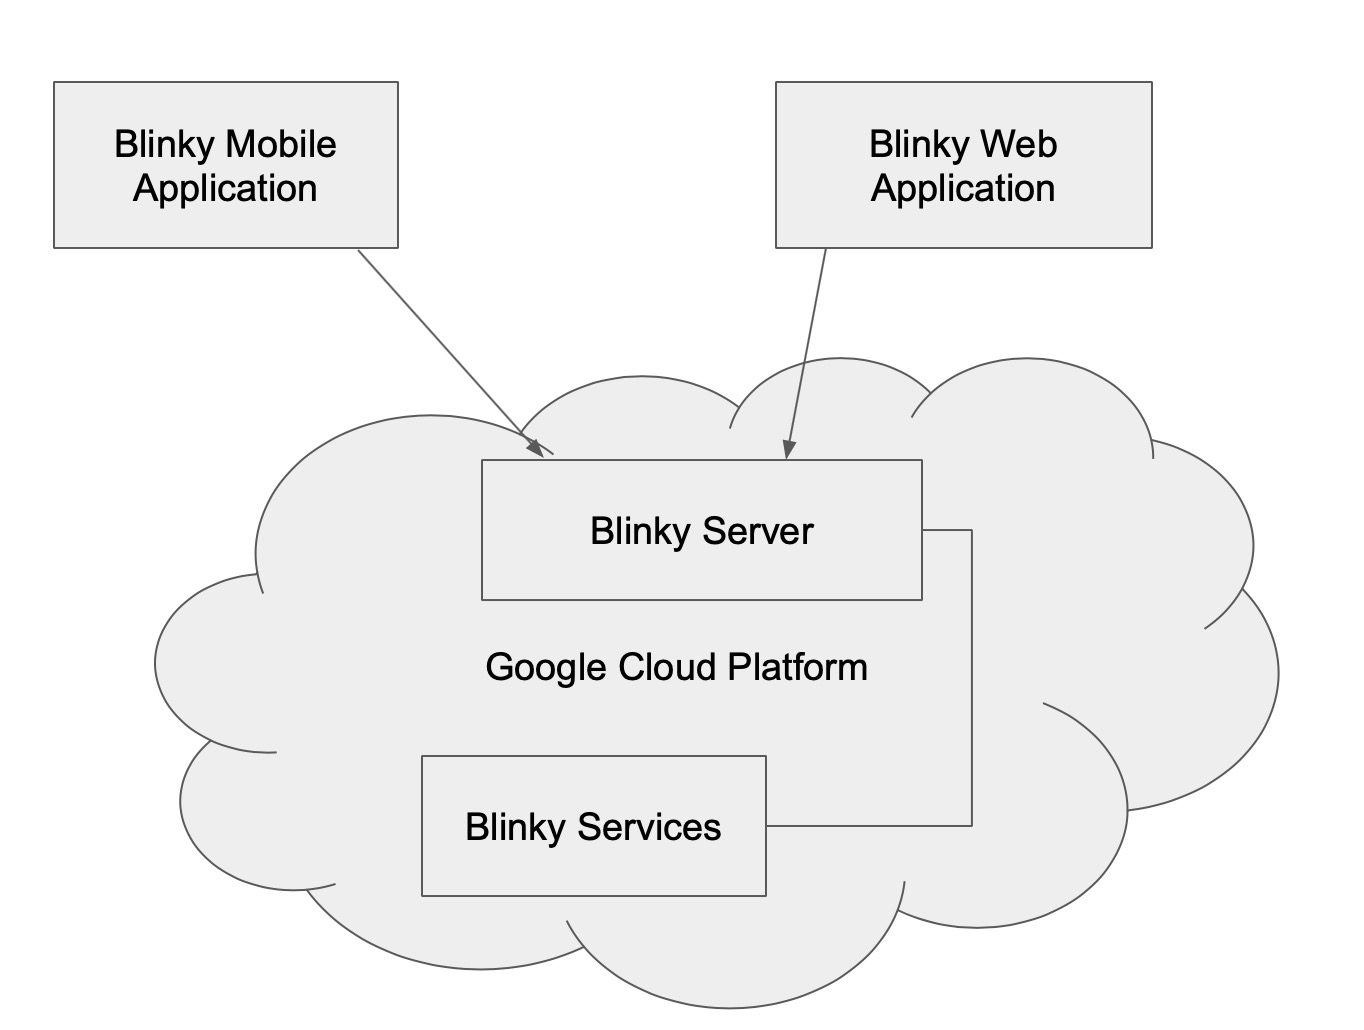
\includegraphics[width=\linewidth]{blinky_system_architecture.jpg}
    \caption{Blinky system architecture}
    \label{fig:blinky_system}
\end{figure}

Users of the Blinky Application can also generate a web URL to share that split cost to friends or relatives. The URL acts as an interface that non-Blinky users can also interact with the services even though they do not have an account. The URL leads to a web application written in React library, which helps building user interface.

Figure \ref{fig:blinky_system} represents the system powering Blinky and where those system are deployed to. 

\section{Application use cases}

The Blinky application was created with the main aim was to help its users to calculate the shares between friends after someone has paid before hand, to ensure a fair and equal split. The application also tries to free users from sticking to one particular payment solution, which allows user to register their preferred payment solution details and later user can share that details together with the calculation details to their friends. Their friends then see the calculation details and take the shared payment method in order to make the payment back to user. From here until the end of this thesis, each of this series of actions from user will be referred as a "cost split" event.

\section{REST API}

The clients, mobile applications and the web application  can communicate with the backend service with a Representational State Transfer (REST)  \citep{REST} Application Programming Interface (API). Data is represented and sent through Javascript Object Notation (JSON).

Users in the mobile application will be granted access right determined by a JSON Web Token (JWT) which can be used in the header of every request to the back-end service. The token contains the user's information which  can easily be used to identify and authenticate them.

The Blinky RestAPI Service will provide an interface for the mobile application so that users can create, edit and delete cost splits, and then invite participants, add expenses to split. Each time a cost split, participant or expense is created on the server, an unique identifier will be generated as an integer and attached to that object. The identifier is then also be used to refer to that object in later actions of its lifetime as well as to delete.
\label{blinkyAPI}

\section{Requirements}
\label{section:requirements}

The requirements for integration with the Ethereum smart contract include:

\begin{itemize}
    \item Generate a new data slot on the smart contract state when a new cost split is created on the application
    \item Increment the data slot with new data each time a cost split is edited with a new user's action such as changing expenses' detail, participants in the cost split, generate an URL, or someone interacted with that URL
\end{itemize}

The requirements are chosen because they depict the common scenarios of transparency between small cost split of a party, such as how much each has to pay, who did declare to have paid.

\subsection{Generating data slot on smart contract}

The desired smart contract will hold a map which contains each cost split's happened event. Each cost split will have its own memory space to store events in a chronological order. Whenever a new event is fired on the client mobile application, a function inside the smart contract should be called provided with the content of the event such as the description, time stamp, user's identifier. The function will then process the input-ed data and append it into that cost split's memory space.

\subsection{Provide a data-retrieval interface for user}

Users of the Blinky application also have the right to request their data in a readable manner, an user-friendly interface. This means that the application will need to provide a function that will represent user and request the data about the user-desired cost split saved on the smart contract. The requested data should also be formatted into a reading-friendly that they can also use as a mean of proof for the action taken by him or anyone interacted with the shared cost split.

\section{Asymptotic Notation}

In order to measure the performance of an algorithm or a computer operation, asymptotic notation is used \citep{AlgorithmAndDataStructure}. In general terms, it is a theoretical framework to measure an algorithm's operation taken to complete the task given a number of inputs. For example, if there is \texttt{n} inputs and the algorithm needs to do \texttt{n} operations on each input, the total number of operations needed to complete the task is \texttt{n * n}, which means it will be exponentially proportional to the number of inputs. In asymptotic notation, only the highest order of operations is taken. From the last example, if the number of operations needed is \texttt{n * n + 2n} then the asymptotic notation is still \texttt{n * n} since it carries order of 2.

\chapter{Implementation}
\label{ch:implementation}

This chapter will describe the proposed solution from this thesis's author for the requirements stated in the previous chapter. This includes explaining the chosen data structure for the smart contract, the framework that was used to connect the smart contract to the Blinky application, the method to validate user's inputs, and potential error handlings.

\section{Smart contract data structure}

In order to write and read cost split data as described in Section \ref{section:requirements}, the data structure of the smart contract will need to be defined. Since each cost split should have its own space to store its event data, one such option for organizing cost splits could be using a \texttt{mapping} \citep{SolidityMapping}. Each cost split will be identified from the key which uses the identifier getting from the Blinky API server as described in Section \ref{blinkyAPI}. This will make cost-split fetching quick and efficient as finding an element in a map knowing its key only need an asymtotic performance of $\Theta(1)$. 

Each event of a cost split will need to carry a description, timestamp, the identifier of the person who initiates the event. Hence, \texttt{struct} data type is the only candidate for defining the data structure of a cost split event. This \texttt{struct} will contains a \texttt{string} type for the description, another \texttt{string} type for the time stamp in the ISO 8601 format \citep{ISOFormat} (such as \texttt{2018-11-12T19:26:47.858Z}) since this format is compatible with various programming languages. The \texttt{struct} will also contain an \texttt{uint} field for storing user's identifier from Blinky API Service. After this passage, the \texttt{struct} will be refered to as \texttt{CostSplitEvent} type.
\label{DataStructure}

Furthermore, after being able to access the data of a cost split using its key, each event should be shorted chronically. Therefore, the option of storing them as an array of \texttt{CostSplitEvent}. Since each event will be recorded chronically by nature, no sorting operation is necessary on the array.

\section{Smart contract functions}

Functions on the smart contract are necessary for interacting with the outer global Internet.

Since the smart contract will need to be able to create a new data slot for a cost split, a function is needed, which can be named as \texttt{createCostSplit}. This function should accept the identifier of the cost split as a parameter and should return a \texttt{boolean} type to indicate if the creation is successful or not, either \texttt{true} or \texttt{false}.

After a cost split is created, users will then began to interact with it in the Blinky Application, which will incur events. Therefore a new function is needed to start to add new event into a cost split. This function can be called \texttt{appendEvent}. In order to identify the cost split and to write the necessary data field of the event as specified in Section \ref{DataStructure}, the function will need to receive the identifier of the cost split, the identifier of the Blinky user initialized the event, time stamp and the event description as the parameter. This function should also denote if the action completes successfully or not so it should return a \texttt{boolean} type like \texttt{createCostSplit}.

Since events happened on a cost split should be persistent due to the reason of transparency, which is the need to get the events and see when a payment is made, accepted or rejected, if a comment into the cost split is made and then deleted, there should not be a function to delete an event of a cost split. This also holds even for the action of deleting a cost split.

\section{Web3 Framework}

After defining the data structure and the functions needed for the smart contract, knowing a tool for communicate with it from the outside Internet is needed. Since the Internet is composed mainly with websites on the browser, such an option for it called the Web3 Framework exist. The advantage of this framework is by written in the pure Javascript language, which is the programming language used in the React Native framework in the Blinky mobile application. This enables fast and easy integration of the framework to both the web page and the mobile application. In order to install and configure the Web3 Framework, there are community composed tutorials, one of which can be found on the web site link: \citep{InstallWeb3}

To conclude the installation of the Web3 Framework process, it consists of the following steps

\begin{itemize}
    \item React Native projects's dependencies can be managed using the \texttt{npm} package manager. Therefore, the content of the Web3 Framework can be downloaded from \texttt{npm}
    \item Choose a suitable Framework version that is compatible with React Native. There are two newest versions: 1.0 and 0.20.x during this time of writing this thesis. Version 1.0's content is generated dynamically, which is not compatible with React Native due to the nature of a mobile application (the code inside the app will be static after being built). Therefore, version 0.22.x is chosen to be installed.
    \item Pony-fill some APIs of Javascript that React Native does not support, such as the \texttt{crypto} API to perform encryption and hashing. Those can be solved by installing package \texttt{node-libs-react-native}
\end{itemize}

After following the mentioned steps and other smaller tweaks in the referral link above. The web3 framwework can be invoked in React Native.

\begin{lstlisting}[float,caption={Calling Web3 functions and making transactions on the Ethereum blockchain \citep{SolidityDocumentation}.},label={lst:callweb3},language=Javascript]

const web3 = new Web3(Web3.givenProvider);
const contractAddress = "0x1a5c29c94D03C4c8f7414564CBD57295d61e898f";
const contractAbi = [
	{
		"constant": false,
		"inputs": [
			{
				"name": "x",
				"type": "uint256"
			}
		],
		"name": "set",
		"outputs": [],
		"payable": false,
		"stateMutability": "nonpayable",
		"type": "function"
	},
	{
		"constant": true,
		"inputs": [],
		"name": "get",
		"outputs": [
			{
				"name": "",
				"type": "uint256"
			}
		],
		"payable": false,
		"stateMutability": "view",
		"type": "function"
	}
];
const myContract = web3.eth.contract(contractAbi);
myContract.methods.myMethod("set")
  .send({from: '0xde0B295669a9FD93d5F28D9Ec85E40f4cb697BAe'})
  .then(function(receipt){})
  .catch(function (error) {});

\end{lstlisting}

In Program \ref{lst:callweb3}, first an instace of the web3 framework is instantiated, with the default provider going together with the framework. Then the contract address contract address and it's Application Binary Interface (ABI) is specified and then be passed to initialize an instace of \texttt{web3.eth.contract}, which represents an Ethereum smart contract. After that, the program can start calling the functions on the smart contract by calling function \texttt{methods.myMethod} on the contract instance.

\section{Error handling}

Error handling is one of the most important aspect when developing a software, to ensure that the software works as expected and maintain a high-quality user experience. In this case of implementing the smart contract for storing cost split event, there are cases which may confuse the smart contract and therefore handling it when making it is a vital step. 

Such errors that can happen are when the smart contract tries to add an event to a non-existing cost split. This kind of error without being handled will result in a malfunctioned application and unexpected user. In this case, since the cost split is not existing, the smart contract should stop the execution of the function and return a \texttt{false} value, so that the clients interacting with the contract is notified that the operation did not succeed, and display the situation on user's device.

\chapter{Evaluation}
\label{ch:evaluation}

This chapter will concentrate on evaluating the smart contract's performance with the mentioned requirement in Chapter \ref{section:requirements}. The evaluation consists of security, privacy, latency and troubleshooting.

\section{Security}
\label{section:security}

Since smart contract is public to the whole blockchain network, there has to be an option to define a rule to execute a function inside a smart contract. Such an option exist in the Solidity language called \textit{function modifier} as mentioned in Section \ref{section:functionModifiers} and a ready-made example in Program \ref{lst:simpleFunctionModifier}. This means the smart contract need to define a modifier that verifies that the function caller is exactly the smart contract owner. To identify who is the owner, the smart contract's constructor need to save the Ethereum address of the caller to one of its own property for later retrieval. This solution provided by Solidity is adequate to protect the smart contract's functions from being called by the unauthorized.

\section{Privacy}

Privacy was not the goal of Ethereum network since every block made in the past can be verified and looked up by the whole network. Therefore, storing the plain data coming from the Blinky application do not provide privacy for user. In order to achieve privacy, the data being sent to smart contract will need to be encrypted. However, a new issue comes up which is who will keep the encryption key. If user is responsible for holding the key, it will require a considerable amount of technical knowledge in order to send and retrieve encrypted data correctly, which will go against the aim of the Blinky application as it tries to provide user the most user-friendly solution. If Blinky application is responsible for holding the encryption key, the aim of decentralized blockchain is also lost since the trust is now given to the Blinky server that it will keep the encryption key secure.

\section{Latency}

The Ethereum network is currently running with the Proof of Work consensus mechanism \citep{RefWorks:doc:BitcoinWhitepaper}, which can only process 15 transactions per second on the whole network, according to the time of writing this thesis. This leads to the unavoided high latency for every time the smart contract is invoked and data is sent. Therefore, interacting with smart contract at this time will not guarantee fast transaction time.

\chapter{Conclusion}
\label{ch:conclusion}

Smart contract can be utilized in social finance application such as the Blinky application which involves in creating and storing event data inside the application. In this work, the Solidity programming language was used to develop a smart contract which acts as a data store for events which happens when user's cost splits incur a new action as mentioned in Chapter \ref{section:requirements}. The language's documentation is well-written and therefore the smart contract was implemented in a short time interval. Since all the transactions happen inside the Ethereum blockchain and with the necessary security action as mentioned in Section \ref{section:security}, it ensures that the data will maintain its integrity, which will be a basis for a potential legal proof in the future.

To build the solution on blockchain also comes with its own cost. Thanks to high latency, users will need to expect longer transaction time in order for their event and data to be written or retrieved. The data that is sent to the smart contract will also not be guaranteed to be private.

With the advantages and disadvantages of a blockchain-based application, this feature of providing user with reliable data source in a smart contract can be released, though not enabled by default. Users can, however, choose to option to each of their own cost split.


%\addto\extrasenglish{\btxifchangecaseoff} % Controls the case-changing for English titles. Make sure that case is preserved for abbreviations and proper nouns, e.g. title={The {ABC} of {Tex}: An Introduction to the Typesetting System}

\ifnameyear
  \bibliographystyle{babapaliktutnat}
\else
  \bibliographystyle{bababbrtut}
\fi
\bibliography{references}


\end{document}